\documentclass{article}

\usepackage[utf8]{inputenc}
\usepackage[english]{babel}
\usepackage{amssymb}
\usepackage{amsthm}
\usepackage{amsfonts}
\usepackage{amsmath}
\usepackage{etoolbox}
\usepackage{enumerate}
\usepackage{breakcites}
\usepackage{float}
\usepackage{algorithm}
\usepackage{algpseudocode, float}
\usepackage{hyperref}
\usepackage{graphicx}

\theoremstyle{definition}
\newtheorem{definition}{Definition}[section]
\AfterEndEnvironment{definition}{\noindent\ignorespaces}

\newtheorem{conjecture}{Conjecture}[section]
\AfterEndEnvironment{conjecture}{\noindent\ignorespaces}

\newtheorem{theorem}{Theorem}[section]
\AfterEndEnvironment{theorem}{\noindent\ignorespaces}

\newtheorem{proposition}{Proposition}[section]
\AfterEndEnvironment{proposition}{\noindent\ignorespaces}

\setlength{\parskip}{.5em}

\title{$k$-Parent Aliquot Numbers: Interm Report Concerning the Image of the Sum-of-Proper-Divisors Function} 
\author{Gavin Guinn\\{\small Supervisor: Michael J. Jacobson}}
\date{December 2021}

\begin{document}
\maketitle
%
%%%%%%%%%%%%%%%%%%%%%%%%%%%%%%%%%%%%%%%%
\section{Introduction}
If we examine numbers in the set $\{6, 28, 496, 8128, ...\}$ we notice that every member $n$ is equal to the sum of its divisors  with the exclusion of itself, 
$$1+2+3 = 6.$$
This of course is the definition of a \textit{perfect number}, a property that has fascinated number theorists since antiquity. The \textit{sum-of-divisors} function is defined for $n > 1$ by
$$\sigma(n) = \sum_{d|n} d.$$
The \textit{proper-divisors} of $n$ refers to the subset of the divisors which excludes itself, the \textit{sum-of-proper-divisors} is defined for $n > 1$ by
$$s(n) = \sigma(n) - n,$$
thus $n$ is a perfect number if and only if $s(n) = n$. The sum-of-proper-divisors is a natural way to consider perfect numbers but is certainly not limited to that domain. For instance consider $s(9) = 4$ which has the property $n < s(n)$, such numbers are \textit{deficient} while numbers that satisfy $n > s(n)$ are \textit{abundant}.

\textit{Aliquot sequences} are produced by iterating $s(n)$, for example consider the sequence starting at $12$:
\begin{align*}
    s(12) &= 1 + 2 + 3 + 4 + 6\\  
    s(16) &= 1 + 2 + 4 + 8\\
    s(15) &= 1 + 3 + 5\\
    s(9) &= 1 + 3\\
    s(4) &= 1 + 2\\
    s(3) &= 1
\end{align*}
In this case the sequence has terminated as $s(n)$ is only defined for $n > 1$, this sequence is also bounded as no value is greater than $16$. A sequence does not have to terminate to be bounded, since perfect numbers are defined by $s(n) = n$ an aliquot sequence that reaches a perfect number will cycle. The members of a cycle of length $2$ are referred to as an \textit{amicable pair}, for instance
$$s(1184) \to s(1210) \to s(1184) \to ...$$
It seems that cycles can form with arbitrary length \cite{chum_guy_jacobson_mosunov_2018} note a cycle of length 24, numbers in such cycles are \textit{sociable}. Aliquot sequences are sometimes said to terminate in a cycle, we will only refer to aliquot sequences that reach $1$ to have terminated while referring to the latter case as a bounded sequence. Aliquot sequences are formalized by \cite{bosma_kane_2010} in the following way:
%
\begin{definition}
The aliquot sequence starting at $a_0 > 1$ is defined by
$$a_0,\text{ }a_1 = s(a_0),\text{ }a_2 = s^2(a_0),\text{ }...$$
\end{definition}
%
\begin{proposition}An aliquot sequence is bounded if and only if 
$$\exists a_n,\,\forall a_m \text{ s.t. }a_n \geq a_m$$  
\end{proposition}
%
The aliquot sequence of 276, 
$$s(276) \rightarrow s(396) \rightarrow s(696) \rightarrow s(1104) \rightarrow s(1872)  \rightarrow ...$$
is the smallest example that has not been shown to be bounded, \cite{zimmermann_2016} has followed the it's growth over 2090 iterations to values with over $200$ digits! The dichotomy between the seemingly unbounded growth of the $276$ sequence and the boundedness of the $12$ sequence gets to the most important open question relating to aliquot sequences:
%
\begin{conjecture}[Catalan-Dickson]
All aliquot sequences are bounded and thus must terminate or enter a cycle. \cite{catalan_1888}
\end{conjecture}
%
\begin{conjecture}[Guy-Selfridge]
The Catalan-Dickson conjecture is false, perhaps most aliquot sequences are unbounded. \cite{guy_selfridge_1975} 
\end{conjecture}
%
The computational exploration of these sequences that has taken place since Catalan originally proposed his conjecture in 1888 has certainly given credence to the Guy-Selfridge point-of-view. However a trend in the data is far from a proof, under our current understanding it is entirely possible that the $276$ sequence could trip over a prime or enter a cycle on some future iteration.
%
\section{Motivation}
What statistics can be compiled on the behaviour of $s(n)$ to argue for or against the Calatan-Dickson Conjecture? The authors of \cite{chum_guy_jacobson_mosunov_2018} consider numerical and analytical approaches to determine the average of $s(n) / n$. The average order of a arithmetic function is a simple function that has the same behaviour on average as the less tractable function. Define $\mathcal{S}(n)$ to be the average order of $s(n)$, when computing the average of $s(n) / n$ we are numerically estimating $\mathcal{S}(n)$. When considering this metric \cite{chum_guy_jacobson_mosunov_2018} restrict the domain to evens to examine $\mathcal{S}(2n)$. I believe the impetus for this decision can be traced to \cite{guy_selfridge_1975} who heuristically argue that unbounded sequences exist:
\begin{itemize}
    \item \textbf{if} $\mathcal{S}(2n) > 2n$ and,
    \item \textbf{if} other effects on the growth of a sequence are relatively minor compared to the tendency for aliquot sequences to preserve parity,
    \item \textbf{then} we would expect most even aliquot sequences that reach large values to be unbounded.
\end{itemize}
This argument seems to match the numerical evidence as seemly unbounded sequences such as $s(276)$ \cite{zimmermann_2016} appear to maintain constant even parity.

The method used to either analytically determine or numerically compute $\mathcal{S}(2n)$ impacts the parameters value. While not explicitly stated by Guy and Selfridge, \cite{bosma_kane_2010} indicate that arithmetic mean of $s(2n) / 2n$ was used to determine $\mathcal{S}(2n)$ in constructing their heuristic argument for unboundedness.
%
\begin{theorem} Arithmetic Mean of $s(2n) / 2n$
$$\lim_{N \to \infty} \frac{1}{N} \sum_{n = 1}^{N} \frac{s(2n)}{2n} = \left(\frac{5\pi^2}{24} - 1\right) = 1.0562...$$
\end{theorem}
%
With this metric we have $\mathcal{S}(2n) = (2n)(1.0563...)$ and thus $\mathcal{S}(2n) > 2n$. However as pointed out by \cite{bosma_kane_2010} the sequence $\{5, \frac{1}{5}, 5, \frac{1}{5}, ... \}$ is bounded but its arithmetic mean tends to $2.6$, a better metric for evaluating the boundedness of a sequence is to consider the geometric mean. 
%
\begin{theorem}Geometric Mean of $s(2n) / 2n$
$$\mu =\lim_{N \to \infty} \exp{\left( \frac{1}{N} \sum_{n=1}^{N} \log s(2n) / 2n \right) =  0.969...}$$
\end{theorem}
%
With this more accurate metric we have $\mathcal{S}(2n) < 2n$ which suggests that even aliquot sequences will in fact decrease on average! This result certainly throws cold water on the heuristic argument of Guy and Selfridge. However the monumental growth of sequences like $s(276)$ suggests that this metric does not completely describe sequence behaviour. 

To improve this model of sequence behaviour the authors of \cite{chum_guy_jacobson_mosunov_2018} consider the image of $s(2n)$ when computing $\mathcal{S}(2n)$. Consider the solutions to $s^{-1}(316),$ 
$$s(192) = s(304) = s(344) = s(412) = 316,$$
since multiple sequences are tributary at $316$ it seems reasonable to conclude that the value of $s(316) / 316$ impacts average sequence growth more than numbers with fewer pre-images. \cite{chum_guy_jacobson_mosunov_2018} explores this by constructing an average of $s(2n)/2n$ weighted by $\#s^{-1}(2n)$. Counting the number of pre-images under $s(2n)$ was certainly on the mind of Dr. Guy when he posed the question that motivates this project:
%
\begin{quote}
Think of a number!! Say $36$\%, which is nice and divisible. It appears that about $36$\% of the even numbers are "orphans".

Divide by 1. For about $36$\% of the (even) values of n there is just one positive integer m such that $s(m) = n$. These values of $n$ have just one "parent".

Divide by 2.  About $18$\% of the even values of $n$ have exactly two parents.

Divide by 3. About $6$\% of the even values of $n$ have three parents.

Divide by 4. About $1.5$\% of the even values of $n$ have just 4 parents.

This suggests that $1 / (e \cdot p!)$ of the even numbers have $p$ parents.

Experiments suggests that these values are a bit large for small values of $p$ and a bit small for larger values of $p$. Can anything be proved?
\end{quote}
%
\begin{definition}
$n$ is a $k$-parent aliquot number if $s^{-1}(n) \text{ has } k \text{ solutions}$.
\end{definition}
%
These percentages refer to the density of even $k$-parent numbers or the probability of encountering a $k$-parent number when choosing randomly from all even natural numbers. There are a suite of colourful names to refer to numbers outside of the range of $s(\cdot)$ including \textit{non-aliquots} and \textit{untouchable numbers}, for the sake of consistency I will be referring to all such numbers as \textit{non-aliquot}.
%
%%%%%%%%%%%%%%%%%%%%%%%%%%%%%%%%%%%%%%%%
\section{Project}
\subsection{Project Preamble}
It is worthwhile to first outline some subtlety around what we are counting when considering $k$-parent numbers and how those counts relate to the existing literature. An important observation when counting non-aliquots is that all odd numbers are in the image of $s(\cdot)$ (with the exception of $5$) \cite{pollPom}, so we only need to consider even numbers when counting non-aliquots. A distinction is that that non-aliquots are numbers outside the image of $s(\cdot)$ while $k$-parent numbers consider how the image of $s(\cdot)$ is distributed. 

In posing his question Dr. Guy considers the density of even $k$-parent numbers over the even numbers.\footnote[1]{This choice may have been made to relate this result back to the Guy-Selfridge heuristic argument for the asymptotic unboundedness of even sequences}\footnote[2]{While it is not the subject of this project it would be perfectly reasonable to consider the the densities of all $k$-parent numbers} This approach differs from that used in the literature around non-aliquots; \cite{chum_guy_jacobson_mosunov_2018}, \cite{pollPom}, and \cite{pomYang} instead consider the density of non-aliquots over all natural numbers. Thus to match the existing literature we will consider the density of \textit{even} $k$-parent numbers over \textit{all natural numbers}. This is slightly awkward as odd $k$-parent numbers exist but we are only considering the density of even $k$-parent numbers over both the evens and odds. However we can take some solace in the fact that densities generated with this method can doubled to convert back to Dr. Guy's approach. A special case to consider is the odd non-aliquot $5$ which will be excluded from the count of even $0$-parent numbers, this will result in such counts being exactly one less than those reported for non-aliquots. With these consideration outlined we can now move to the project particulars.

\subsection{Previous Work}
It is useful to observe that $k$-parent aliquot numbers are a generalization of non-aliquots. Thus an effective strategy for quantifying the density of $k$-parent numbers is to generalize techniques such as the heuristic approach of \cite{pollPom}. The authors employ statistical methods to model the density of non-aliquots, this model closely matches experimental observations.
% 
\begin{conjecture}{Heuristic Model for the Density of Non-Aliquots}
$$\Delta = \lim_{y \to \infty}\frac{1}{\log y} \sum_{\substack{a\leq y \\ 2 | a}} \frac{1}{a}\text{e}^{-a/s(a)}$$
\end{conjecture}
%
During a previous work term I produced the following tentative generalization of this model.
%
\begin{conjecture}{Heuristic Model for the Density of Even $k$-Parent Numbers}
$$\Delta_k = \lim_{y \to \infty} \frac{1}{\log y}\sum_{\substack{a \leq y \\ 2 | a}} \frac{a^{k-1}}{k! \cdot s(a)^k} \cdot \text{e}^{-a/s(a)}$$
\end{conjecture}
%
A priority for this project is to fully justify this result. Some values are given in Table \ref{tab:hueristic-dr.guy}.
%
\begin{table}[H]
 	\centering
    \begin{tabular}{| c | c | c | c | c | c |}
      \hline
      $\Delta_k$     &   $k = 0$  &   $k = 1$  &   $k = 2$  &   $k = 3$  &   $k = 4$  \\ 
        \hline
        $y = 10^3$  &   0.155   &   0.164   &   0.100   &   0.046   &   0.018   \\
        $y = 10^4$  &   0.161   &   0.165   &   0.098   &   0.044   &   0.017   \\
        $y = 10^5$  &   0.165   &   0.166   &   0.097   &   0.044   &   0.016   \\
        $y = 10^6$  &   0.167   &   0.166   &   0.096   &   0.043   &   0.016   \\
        $y = 10^7$  &   0.169   &   0.167   &   0.096   &   0.042   &   0.016   \\
      \hline
      \hline
      \hline
      $1/(p! \cdot \text{e})$   &   $p = 0$ &   $p = 1$ &   $p = 2$ &   $p = 3$    &   $p = 4$ \\
      \hline
      - &   0.378   &   0.368   &   0.184   &   0.061   &   0.015   \\
      \hline
      \hline
      $1/2(p! \cdot \text{e})$  &   $p = 0$ &   $p = 1$ &   $p = 2$ &   $p = 3$    &   $p = 4$ \\
      \hline
      -     &   0.184   &   0.184   &   0.092   &   0.031   &   0.008   \\
      \hline
	\end{tabular}
    \caption{Approximation of $\Delta_k$ compared to Dr. Guy's estimates}
    \label{tab:hueristic-dr.guy}
\end{table}
%
A complementary approach is to directly compute the densities of $k$-parent numbers. If the computed densities closely match the heuristic model we would have strong evidence for correctness. \cite{chum_guy_jacobson_mosunov_2018} leverage an algorithm of \cite{pomYang} to enumerate the image of $s(2n)$ within a bounding range, the percentage of numbers in this range that are not enumerated is the density of non-aliquots. During that previous work term I successfully generalized this technique to compute the densities of $k$-parent numbers, however this code is currently bugged such that the counts of $0$-parent numbers diverge from the published counts of non-aliquots at the bound of $2^{40}$. Densities computed by this program are compared to values of $\Delta_k$ and Dr. Guys estimates in Table \ref{tab:computed}.
%
\begin{table}[H]
    \centering
    \begin{tabular}{| c | c | c | c | c | c |}
        \hline
        $a_k(n) / n$   &   $k = 0$     &   $k = 1$     &   $k = 2$     &   $k = 3$     &   $k = 4$     \\ 
        \hline
        $n = 10^3$  &   0.088    &  0.202   &   0.148    &   0.048    &  0.009    \\
        $n = 10^4$  &   0.121    &  0.187   &   0.121    &   0.048    &  0.015    \\
        $n = 10^5$  &   0.139    &  0.182   &   0.108    &   0.045    &  0.016    \\
        $n = 10^6$  &   0.150    &  0.178   &   0.103    &   0.042    &  0.016    \\
        $n = 10^7$  &   0.157    &  0.175   &   0.099    &   0.042    &  0.016    \\
        $n = 10^8$  &   0.162    &  0.173   &   0.097    &   0.041    &  0.016    \\
        $n = 10^9$  &   0.166    &  0.171   &   0.096    &   0.040    &  0.015    \\
        \hline
        \hline
        \hline
        $y$     &   $\Delta_0$  &   $\Delta_1$  &   $\Delta_2$  &   $\Delta_3$  &   $\Delta_4$  \\
        \hline
        $y = 10^7$  &   0.169   &   0.167   &   0.096   &   0.042   &   0.016   \\      
        \hline
        \hline
        \hline
        $1/2(p! \cdot \text{e})$   &   $p=0$    &   $p=1$    &   $p=2$    &   $p=3$   &   $p=4$    \\
        \hline
        -     &   0.184   &   0.184   &   0.092   &   0.031   &   0.008   \\
        \hline
    \end{tabular}
    \caption{$a_k(n)$ is a counting function for $k$-parent aliquot numbers less than or equal to $n$, $a_k(n) = |\{x \,| \, \#s(x)^{-1} = k,\, 1 \leq x \leq n\}|$.}
    \label{tab:computed}
\end{table}

\subsection{Project Goals}
The goals for this project are: \begin{enumerate}
    \item Correct my previous implementation of the Pomerance-Yang (P-Y) algorithm \cite{pomYang} that produced a off-by-one error at bound $2^{40}$. Steps in this debugging process include: \begin{enumerate}[(a)]
        \item Ensure correctness of $\sigma(\cdot)$ enumeration which is required by the P-Y algorithm. I will compare the outputs of this implementation with other algorithms for enumerating $\sigma(\cdot)$ up-to $2^{40}$. If multiple distinct algorithms produce identical output we will have reasonably strong evidence for the enumerations correctness.
        \item If the above method does not identify the source if the bug I will compare the intermediate results of my implementation of P-Y with the implementation used in \cite{chum_guy_jacobson_mosunov_2018}. This could be done by running the implementations in parallel and comparing the characteristic functions after each block is completed. This computationally and memory expensive method would certainly identify the value in which the implementations differ. 
    \end{enumerate}
    \item Formalize the argument justifying my generalization of the heuristic model of \cite{pollPom} for approximating the density of non-aliquot numbers. It remains to ensure correctness of my argument and rewrite in a formal style.
    \item A related goal to correcting my P-Y implementation of is to tune the inputs to ensure optimal performance. For instance setting the length to be sieved over in a step incorrectly can result in an order-of-magnitude increase in run-time. Choosing optimized values for all these constants in a multi-threaded context is non-trivial and would likely involve tuning to the specifications of the hardware running the algorithm (i.e. CPU cache).
    \item A secondary goal to correcting my implementation of P-Y is to research alternative algorithms for enumerating the sum-of-proper divisors. This algorithm dominates the run-time of P-Y so improvements are highly desirable.
    \item A small side goal is to recompute the weighted geometric mean of $s(n)/n$ weighted by $1$ if $n$ is an aliquot orphan and $\#s^{-1}(n)$ otherwise. The rational for this is explained in \autoref{sec:chumetal}.
    \item If time allows I will seek to generalize the provable lower bounds of \cite{chen_zhao_2011} for the density of non-aliquot numbers. I would generalize this work to prove lower bounds for the densities of $k$-parent numbers.
\end{enumerate}
The final goal of the project is to produce a paper that presents my heuristic model for $k$-parent numbers and utilizes the computed densities of $k$-parent as evidence for that result. The correctness of computational work will be thoroughly tested and the code will be available in a well-documented GitHub repository. This work will be motivated in the context of Dr. Guy's original problem statement and the Guy-Selfridge conjecture in general.

\subsection{Project Status}
The bulk of my time on this project has been spent reviewing the related literature, this context will certainly be useful when preparing the final report. I have also spent a good deal of time developing an algorithm for enumerating ranges of $\sigma(\cdot)$ similar to that of \cite{moews_moews_1991}, a discussion these algorithms and the relationship to P-Y can be found in \autoref{sec:ennum}. This algorithm could be useful in checking the correctness of the implementation I inherited from another researcher. This effort has given me experience working with sieving algorithms and insight into the challenges of tuning them for optimal performance.

I have also re-familiarized myself with my implementation of P-Y and attempted to re-run it on ARC, uCalgary's high performance cluster. The jobs I have submitted at bounds $10^{12}$ and $2^{40}$ have so far been unsuccessful due to either exceeding time or memory constraints, a priority is to reproduce the erroneous computation as a first step in debugging the error.

\subsection{Project Timeline}
I will to reproduce the erroneous computation as soon as possible; the delays associated with batch processing queues and the long computation time needed are the primary challenges to this deliverable. I will also confirm the correctness of the $\sigma(\cdot)$ enumeration as soon as possible, my work on an alternative $\sigma(\cdot)$ enumeration has already produced much of the computational machinery needed to do this. During the winter break I will take some time to compile all the disparate programming and writing I have produced so far into a single well-documented GitHub repository. Also during the break I will have a developed a method to tune this algorithm to ensure near optimal performance and memory usage. 

Early in the winter semester, mid January 2022, I hope to have resolved the bug in my implementation of the P-Y algorithm. At a minimum by this point I will have compared my implementation of P-Y with that used in \cite{chum_guy_jacobson_mosunov_2018} and determined the value where the implementations vary. At this point I also will have computed the alternative geometric mean of $s(n)$ described above.

By the start of February 2022 I hope to have my work on the $k$-parent heuristic model summarized into a form appropriate for the final report. This will involve communicating with my supervisor to determine what details need to be included and what mathematical correctness issues need to be addressed. 

Once these goals are achieved I will start writing my final paper and presentation which will summarize my effort on this project over both my NSERC work-term and the 502 course. If time allows I will explore either the provable lower bounds of \cite{chen_zhao_2011} or faster algorithms for enumerating $\sigma(\cdot)$.  

\section{Discussion of Algorithms}
\label{sec:ennum}
To compute the density of k-parent aliquot numbers up-to bound $X$ we must enumerate the image of all values $n$ such that $s(n) \leq X$. For each $m \leq X$ we will have computed $k$ distinct values of $n$ such that $s(n) = m$, more concisely $s^{-1}(m) = \{n\,|\,s(n) = m\}$ and thus $$\#s^{-1}(m) = |\{n\,|\,s(n) = m\}|.$$ $\#s^{-1}(m)$ is computed by looping through all values $m$ corresponding to the previously enumerated $n$ and iterating a counter in a array index corresponding to $m$.

The P-Y algorithm, described in \autoref{sec:pomyang}, is utilized to compute $s^{-1}(m)$. This algorithm requires $\sigma(n)$ for every odd value $n$ between 1 and the upper bound $X$. Perhaps the simplest implementation is to directly compute these values of $\sigma(n)$ by directly factoring each value $n$ using an approach like Pollard's Rho algorithm, however this approach is untenable at higher bounds. Sieving algorithms which produce enumerated ranges of $\sigma(\cdot)$ have a significant run-time advantage compared to enumerating a range with a one-at-a-time factoring algorithm.

\subsection{Moews and Moews Algorithm for Enumerating $\sigma(\cdot)$}
The current state-of-the-art for enumerating $\sigma(\cdot)$ is the segmented sieving algorithm of \cite{moews_moews_1991}, Algorithm \autoref{alg:M-M} is a transcription into pseudo-code. I believe this algorithm leverages the multiplicative property of $\sigma(\cdot)$ \cite{2021Multiplicative} to compute values as a product where $p$ is prime and $n =p^{a_1}_{1}p^{a_2}_{2}\,...\, p^{a_t}_{t}$, $$\sigma(n) = \sigma(p^{a_1}_{1}) \sigma(p^{a_2}_{2}) \,...\,\sigma(p^{a_t}_{t}).$$  This strait-forward implementation of Moews and Moews (M-M) is inefficient, seemly due to the test on line 9 failing for most values of $j$. I inherited an optimized version of this algorithm that was used in \cite{chum_guy_jacobson_mosunov_2018} which seems to improve run-time shape; while I don't entirely understand the technique but it seems to reduce the number of tests by offsetting to values guaranteed to be divisible by $p^e$.

I cannot perform a direct performance comparison between the optimized and optimized implementations of M-M as I am not in possession of equivalent working implementations. However I do have working implementations of naive M-M and a inherited implementation of optimized M-M which enumerates $\sigma(n)$ for odd values of $n$; \autoref{tab:M-Mtiming} presents a timing comparison to roughly demonstrate the need for optimization in making M-M performant.   

\begin{algorithm}[H]
\caption{M-M Algorithm to Enumerate Range of $\sigma(\cdot)$} 
\begin{algorithmic}[1]
    \Procedure{enumerate sigma}{$N,\,M$} \Comment{$N$ is length, $M$ is base}
    \State $q[j] \gets j + M,\, \forall j \in [0,\, N-1]$
    \State $r[j] \gets 1,\, \forall j \in [0,\,  N-1]$
    \ForAll{primes $p \leq \sqrt{M+N-1}$}
        \State $p^e \gets p$
        \While{$p^e \leq M + N$}
            \State $p^{e+1} \gets p^e \cdot p$
            \ForAll{$\forall j \in [0,\, N-1]$}
                \If{$p^e\,|\,(M + j)$ and $p^{e+1}\nmid (M + j)$}
                    \State $q[j] \gets q[j] / p^e$
                    \State $r[j] \gets r[j] \cdot ((p^{e+1} - 1) / (p - 1))$ \Comment{$r[j] = r[j] \cdot \sigma(p^e)$}
                \EndIf
            \EndFor
            \State $p^e \gets p^{e+1}$
        \EndWhile
    \EndFor
    \ForAll{$\forall j \in [0,\, N-1]$}
        \If{$q[j] \neq 1$}
            \State $r[j] \gets r[j] \cdot (q[j] + 1)$
        \EndIf
    \EndFor
    \State \textbf{return} $r$
    \EndProcedure
\end{algorithmic}
\label{alg:M-M}
\end{algorithm}

\begin{table}[H]
    \centering
    \begin{tabular}{| c | c | c |}
        \hline
        -   &   Naive M-M     &   Optimized Odd M-M \\ 
        \hline
        $X = 10^4$  &   0.01s    &  0.00s  \\
        $X = 10^5$  &   0.07s    &  0.01s  \\
        $X = 10^6$  &   1.35s    &  0.04s  \\
        $X = 10^7$  &   32.69s    & 0.36s  \\
        \hline
    \end{tabular}
    \caption{Timings comparison between naive M-M and optimized odd M-M, sieving $\sigma(\cdot)$ to bound $X$.}
    \label{tab:M-Mtiming}
\end{table}

\subsection{Segmented Accumulating Sieve for Enumerating $\sigma(\cdot)$}
Before studying the M-M algorithm I implemented similar style of segmented sieve that computes enumerates $s(\cdot)$ from 1 to bound $X$ such that the memory requirements are proportional to $\sqrt{X}$. This algorithm operates on a similar principle to the segmented sieve of Eratosthenes but instead of marking a number with a divisor non-prime it instead accumulates the divisor, I will refer to this as the segmented accumulating sieve (SAS) algorithm. The pseudo-code can be found in Algorithm \autoref{alg:SAS}.

Note that the SAS algorithm only enumerates $s(\cdot)$ between 1 and $M$ while M-M can enumerate any selected range of $\sigma(\cdot)$. This is because the SAS algorithm relies on the state of buffers $s$ and $i$ to compute the next block. This is possibly correctable utilizing a trick to find the offset $m + X$ of a number $n$ above a bound $X$, $$m = (n - (X \,\text{mod}\, n)) \,\text{mod}\, n,$$ which I found in the optimized M-M implementation.

I cannot perform a direct performance comparison between the SAS algorithm and optimized implementations of M-M as I am not in possession of equivalent working implementations. However I can compare my SAS implementation which enumerates all $s(\cdot)$ up-to bound $X$ with the optimized odd M-M which enumerates odd $\sigma(\cdot)$, this is presented in \autoref{tab:SAStiming}. Based on this limited experimental evidence it appears that both algorithms are linear to $X$ with optimized odd M-M faster by a constant factor of 2; this constant run-time difference might be a result of optimized odd M-M sieving exactly half as many numbers as SAS.

An size of block being sieved over in a given step, $B$ for Algorithm \autoref{alg:SAS} and $N$ for Algorithm \autoref{alg:M-M}, have dramatic performance implications. Timing and buffer use information for the SAS algorithm at various values of $B$ are given in \autoref{tab:SAStuning}. The poor timings for $10^2$ and $10^3$ can likely be attributed to the algorithm spending to much time on loop controlling operations. The timings for $10^4$ to $10^6$ are all roughly similar, I hypothesize that this is because the buffers for these values sit comfortably in my CPU's 32 MiB L3 cache; I suspect the timings jump again at $10^7$ because the buffer cannot all be cached simultaneously.   
\begin{algorithm}[H]
\caption{SAS Algorithm to Enumerate $s(\cdot)$} 
\begin{algorithmic}[1]
    \Procedure{enumerate sn}{$M,\,B$} \Comment{$M$ is max, $B$ is block length}
    \State $s[i] \gets 0,\, \forall i \in [0,\, B - 1]$
    \State $t[i] \gets 1,\, \forall i \in [0,\, \sqrt{M}]$ \Comment{iterations buffer}
    \State $m[i] \gets i,\, \forall i \in [0,\, \sqrt{M}]$ \Comment{multiple buffer}
    \ForAll{$i \in [B,\, 2B,\, ...\,,\, M]$}
        \State $d \gets \sqrt{M}$ \Comment{max divisor}
        \While{$d \geq 1$}
            \ForAll{$j \in [1, d]$}
                \If{$m[j] \leq i$}
                    \State $N \gets m[j] - (i - B + 1)$ \Comment{offsetting}
                    \State $s[N] \gets s[N] + j$
                    \If{$t[j] > \sqrt{M}$}
                        \State $s[N] \gets s[N] + t[j]$ \Comment{accumulate divisor's pair}
                    \EndIf
                    \State $t[j] \gets t[j] + 1$
                    \State $m[j] \gets m[j] + j$
                \EndIf
            \EndFor
            \While{$m[d] > i$}
                \State $d \gets d - 1$
            \EndWhile
        \EndWhile
        \State $s[j] \gets 0,\, \forall j \in [0,\, B - 1]$ \Comment{offload range before clearing}
    \EndFor
    \EndProcedure
\end{algorithmic}
\label{alg:SAS}
\end{algorithm}

\begin{table}[H]
    \centering
    \begin{tabular}{| c | c | c |}
        \hline
        -   &   SAS    &   Optimized Odd M-M \\ 
        \hline
        $X = 10^6$  &   0.08s    &  0.04s  \\
        $X = 10^7$  &   0.75s    &  0.36s  \\
        $X = 10^8$  &   8.20s    &  3.45s  \\
        $X = 10^9$  &   83.22s    &  47.17s  \\
        \hline
    \end{tabular}
    \caption{Timings comparison between SAS algorithm and optimized odd M-M, sieving $s(\cdot)$ and $\sigma(\cdot)$ respectively to bound $X$.}
    \label{tab:SAStiming}
\end{table}

\begin{table}[H]
    \centering
    \begin{tabular}{| c | c | c |}
        \hline
        SAS ($M = 10^8$)   &    Timing   &  $s[i]$ Buffer size \\ 
        \hline
        $B = 10^2$  &   18.14s    &  0.78 KiB  \\
        $B = 10^3$   &   9.23s    &  7.81 KiB  \\
        $B = 10^4$   &   8.43s    &  78.13 KiB  \\
        $B = 10^5$   &   8.62s    &  0.76 MiB  \\
        $B = 10^6$   &   8.70s    &  7.63 MiB  \\
        $B = 10^7$   &   17.38s    &  76.29 MiB  \\
        $B = 10^8$   &   18.91s    &  762.9 MiB  \\
        \hline
    \end{tabular}
    \caption{Timings and $s$ buffer sizes used by the SAS algorithm at different values of $B$.}
    \label{tab:SAStuning}
\end{table}


\section{Review of Related Works}
%
%%%%%%%%%%%%%%%%%%%%%%%%%%%%%%%%%%%%%%%%
\subsection{Variant of a Theorem of Erdős on the Sum-of-Proper-Divisors Function}
\label{sec:pomyang}
The authors of \cite{pomYang} are principally concerned with establishing upper and lower bounds on the density of numbers outside of the range of the \textit{sum-of-unitary divisors} function, defined for all natural numbers by: 
$$\sigma^*(n) = \sum_{\substack{d | n \\ \gcd(d,n/d) = 1}} d.$$
This variant of the sum-of-divisors only sums divisors $d$ that are co-prime with $d/n$. The authors also discuss previous analytic results on numbers outside of the range $\phi(n)$ and $s(n)$.   $\phi(n)$ referring to \textit{Euler's phi function} which counts positive integers $k \leq n$ such that $k$ is co-prime with $n$, where $k$ and $n$ are co-prime if $\gcd(k, n) = 1$. Of particular interest to this project the authors also present a set of nearly linear algorithms to enumerate values outside the image of $s(n)$, $n - \phi(n),$ and $\sigma^*(n) - n$ within a bound.

The authors discuss a previously mentioned property that almost every odd number is in the image of $s(\cdot)$ thus when studying non-aliquots we need only consider even numbers. This follows from a stronger form of the Goldbach conjecture which states that all even $m \geq 8$ there exists distinct primes $p$ and $q$ such that $m = p+q$. Noting that the only proper divisors of a product of primes are those primes and $1$, $$s(pq) = p + q + 1 = m + 1$$ thus covering every odd number greater than or equal to $9$. We have that $5$ is the only odd non-aliquot as $s(4) = 3$, $s(8) = 7$, and $s(p) = 1$ where $p$ is any prime.

The algorithm presented for the enumeration of non-aliquots within a bound is of key importance for this project, this will be referred to as the \textit{Pomerance-Yang (P-Y) algorithm}. When enumerating non-aliquots it is useful to consider cases where $s(\cdot)$ maps to an even number.
\begin{proposition}
    $s(n)$ is even if and only if
    \begin{enumerate}[(i)]
        \item $n = (2m+1)^2$, or
        \item $2 | n$ and $(n \neq m^2 \text{ or } n \neq 2m^2)$.
    \end{enumerate}
\end{proposition}

We can observe that parity only flips when squares are encountered, it is worth outlining the intuition on why this is the case. Notice that a non-square necessarily must have a odd number of proper divisors as we include $1$ and some number of factor pairs. However a square $n$ must an even number of proper divisors as we include $1$, $\sqrt{n}$, and some number of factor pairs. $(2m+1)^2$ will have an even count of strictly odd proper-divisors, the sum of such a set of numbers will have even parity. The even case seems to be a slightly more involved exercise, a discussion of this in the context of $\sigma(\cdot)$ is presented by \cite{sumdiv_odd}. 

The P-Y algorithm employs this property to split the computation of the even image of $s(\cdot)$ into distinct cases. For the even case the authors construct a recurrence from the following proposition.
\begin{proposition}
    Let $j$ be a positive integer and $m$ be an odd positive integer, the following statements hold:
      \begin{enumerate}[(i)]
        \item $s(2m) = 3\sigma(m) - 2m$,
        \item $s(2^{j+1}m) = 2s(2^{j}m) + \sigma(m)$.
    \end{enumerate}
\end{proposition}
The multiplicative property of the $\sigma(\cdot)$ \cite{2021Multiplicative} gives context to how these statements where constructed. For the odd case the image of numbers $p^2$ for some prime $p < x$ are detected within the same loop as the recurrence while $m^2$ for some odd composite $m < x^{2/3}$ are computed separately. Non-aliquots are numbers within the range that have not been touched by the enumeration.

Since the P-Y algorithm for $s(\cdot)$ was described in comparison to similar algorithms I will outline this version as a stand-alone algorithm.
\begin{algorithm}[H]
\caption{P-Y Algorithm to Enumerate Non-Aliquots} 
\begin{algorithmic}[1]
    \Procedure{enumerate non aliquots}{$x$}
    \State{$f[i] \gets 1,\, \forall i \in [1, x]$}
    \ForAll{odd $m \in [1, x]$}
        \If{$2 | \sigma(m)$}
            \State $t \gets 3\sigma(m) - 2m$
            \While{$t \leq x$}
                \State{$f[t] \gets 0$}
                \State{$t \gets 2t + \sigma(m)$}
            \EndWhile
        \EndIf
        \If{$\sigma(m) = m+1$} \Comment{if $m$ is prime}
            \State{$f[m+1] \gets 0$}
        \EndIf
    \EndFor
    \ForAll{odd composite $m \in [1, x^{2/3})$}
        \If{$s(m^2) \leq x$}
            \State{$f[s(m^2)] \gets 0$}
        \EndIf
    \EndFor
    \State{\textbf{return} $f$}
    \EndProcedure
\end{algorithmic}
\end{algorithm} 
%%% not presenting as i couldn't prove (ii)
% \noindent(i)
% \begin{align*}
%     s(2m) &= \sigma(2m) - 2m \\
%     &= \sigma(2)\sigma(m) - 2m  & \text{note: } 2 \nmid m \\
%     &= 3\sigma(m) - 2m
% \end{align*}
%
%%%%%%%%%%%%%%%%%%%%%%%%%%%%%%%%%%%%%%%%
\subsection{Some Problems of Erdős on the Sum-of-Divisors Function}
%
\cite{pollPom} tackle 3 problems regarding the sum-of-divisors function: bounding the number of aliquot reversals, bounding the number friendly pairs, and of specific interest developing a heuristic model for the density of non-aliquots. Contextually this paper largely engages with problems proposed by Erdős with an eye for relating the results back to the Guy-Selfridge / Catalan-Dickson conjectures.

Aliquot sequences have a tendency to preserve abundancy or deficiency, an aliquot reversal a number where this tendency does not hold. These reversals are of key importance when considering amicable pairs or sociable numbers more generally, these cycles require a reversal of abundancy to form. Take the following amicable pair for example:
\begin{align*}
    s(220) = 284 & \textit{ up-down reversal}\\
    s(284) = 220 & \textit{ down-up reversal}
\end{align*}
The authors note a result of Erdős who by proving that there are few up-down reversals was able to establish that the numbers involved in amicable pairs (later extended to sociable numbers) have a vanishing asymptotic density. With this an analog of the Guy-Selfridge heuristic argument for sequence unboundedness is presented:
\begin{itemize}
    \item \textbf{if} aliquot sequences tend to preserve parity, and
    \item \textbf{if} sociable cycles are of vanishing density, and
    \item \textbf{since} a sequence is only bounded if it enters a cycle or terminates on a prime;
    \item \textbf{then} even sequences tend to be unbounded.
\end{itemize}
However the authors point out the result of \cite{bosma_kane_2010} who demonstrated that on average even numbers tend to be slightly deficient, as such under this argument we would expect even sequences to be bounded.

While not a direct response to the text this line-of-reasoning did prompt me to consider the purpose of this style of heuristic argument more generally. If we assume that $\mathcal{S}(2n) < 2n$ we would not have a proof that all even sequences will terminate. For demonstrative purposes consider a toy function defined by:
$$r(n) = 
\begin{cases} 
    10n & \text{if } n = 10^m \\
    1 & \text{otherwise}
\end{cases}$$
Sequences generated by iterating this function will be unbounded only if $n$ is a power of $10$. Based on some quick numerical estimation it seems the geometric mean of $r(n) / n$ tends towards $0$. This demonstrates the possibility that some subset of sequences can be unbounded while on average sequences tend to decrease. I am not sure if it is possible to construct an analogous example where the geometric mean of $r(n)/n$ is greater than 1 but every sequence is bounded. 

$30$ and $120$ are examples of numbers that share the same ratio $\sigma(n)/n$, such numbers are known as \textit{friendly pairs},
$$\frac{\sigma(30)}{30} = \frac{12}{5} = \frac{\sigma(120)}{120}.$$
The authors prove bounds on how many numbers satisfy a slightly stronger condition of \textit{primitive friendly pairs}. While not a direct response to the text it is interesting to note that the concept of friendly pairs and more generally \textit{friendly clubs} might be useful when storing a computed range of $\sigma(n)$. Storing $\sigma(n)/n$ instead could possibly reduce the number of bits needed and the presence of friendly clubs introduces repetition which would improve data compression ratios.

Most relevant for my project the authors construct a heuristic model for the density of non-aliquots,
$$\Delta = \lim_{y \to \infty}\frac{1}{\log y} \sum_{\substack{a\leq y \\ 2 | a}} \frac{1}{a}\text{e}^{-a/s(a)}.$$
The bulk of my previous work term was spent in generalizing this result into Conjecture 1.2. In brief this model was constructed by setting up the relevant criteria and assumptions to apply the "balls and bins" statistics problem to estimate the number of non-aliquots. We consider the results of $s(n)$ as the thrown balls and some well defined subset of the even numbers as the bins. Say you have $n$ bins and toss $m$ balls, we can compute the probable number of empty bins after this process with: $$\# [\text{empty bins}] = n(1- \frac{1}{n})^m.$$
The number of "empty bins" thus estimates the number of non-aliquots.
%
%%%%%%%%%%%%%%%%%%%%%%%%%%%%%%%%%%%%%%%%
\subsection{Numerical and Statistical Analysis of Aliquot Sequences}
\label{sec:chumetal}
\footnote{My initial draft at reviewing \cite{chum_guy_jacobson_mosunov_2018} was largely edited into the motivation section of this paper. Unfortunately due to time constraints I was unable finish this review, however I believe this isolated point is interesting enough to leave in.}
In \cite{chum_guy_jacobson_mosunov_2018} the weighted geometric mean of $s(n)/n$ is computed with each ratio weighted by $\#s^{-1}(n)$, the idea being that numbers with many parents have a larger impact on the average behaviour of sequences. This method gives $0$ weight to $s(n)/n$ for $\#s^{-1}(n) = 0$, however non-aliquot numbers can be thought of as the start of sequences rather than numbers excluded from sequences. This is necessarily true, if some number $n$ has $\#s^{-1}(n) > 0$ then there must be some preceding number in the same sequence, an non-aliquot is where this recursion terminates. Consider the sequence originating at the non-aliquot $52$: 
$$s(52) \to s(46) \to s(26) \to s(16) \to s(15) \to s(9) \to s(4) \to s(3) \to s(1)$$It seems to me that $s(52)/52$ has no less impact on the termination than any other number in the sequence. Perhaps non-aliquots should be considered with weight $1$ when computing such an average.
%
%%%%%%%%%%%%%%%%%%%%%%%%%%%%%%%%%%%%%%%%
\section{Conclusion}
My project on computationally and heuristically quantifying the densities of $k$-parent aliquot numbers fits best into existing literature when discussed in the context of the Guy-Selfridge conjecture. In this approach the conjecture is best viewed as a way to inspire new and creative mathematics rather than a statement that urgently requires a proof. With this mindset I hope this work might be able to add some interest into the heuristic discussion of Guy-Selfridge.

Elaborating the discussion around $k$-parent numbers could enable further explorations into more general \textit{aliquot genealogies}, just as the generalization of non-aliquots enabled this project. By this I am referring to the idea an aliquot number also has some number of \textit{grand-parents} or in other words the number of sequences tributary to a number $2$ pre-images removed, \autoref{fig:geno} provides an illustration of this concept. It is possible that such considerations could provide an interesting way to model sequence behaviour.

% \begin{figure}[t]
% \caption{Example of a parametric plot ($\sin (x), \cos(x), x$)}

% 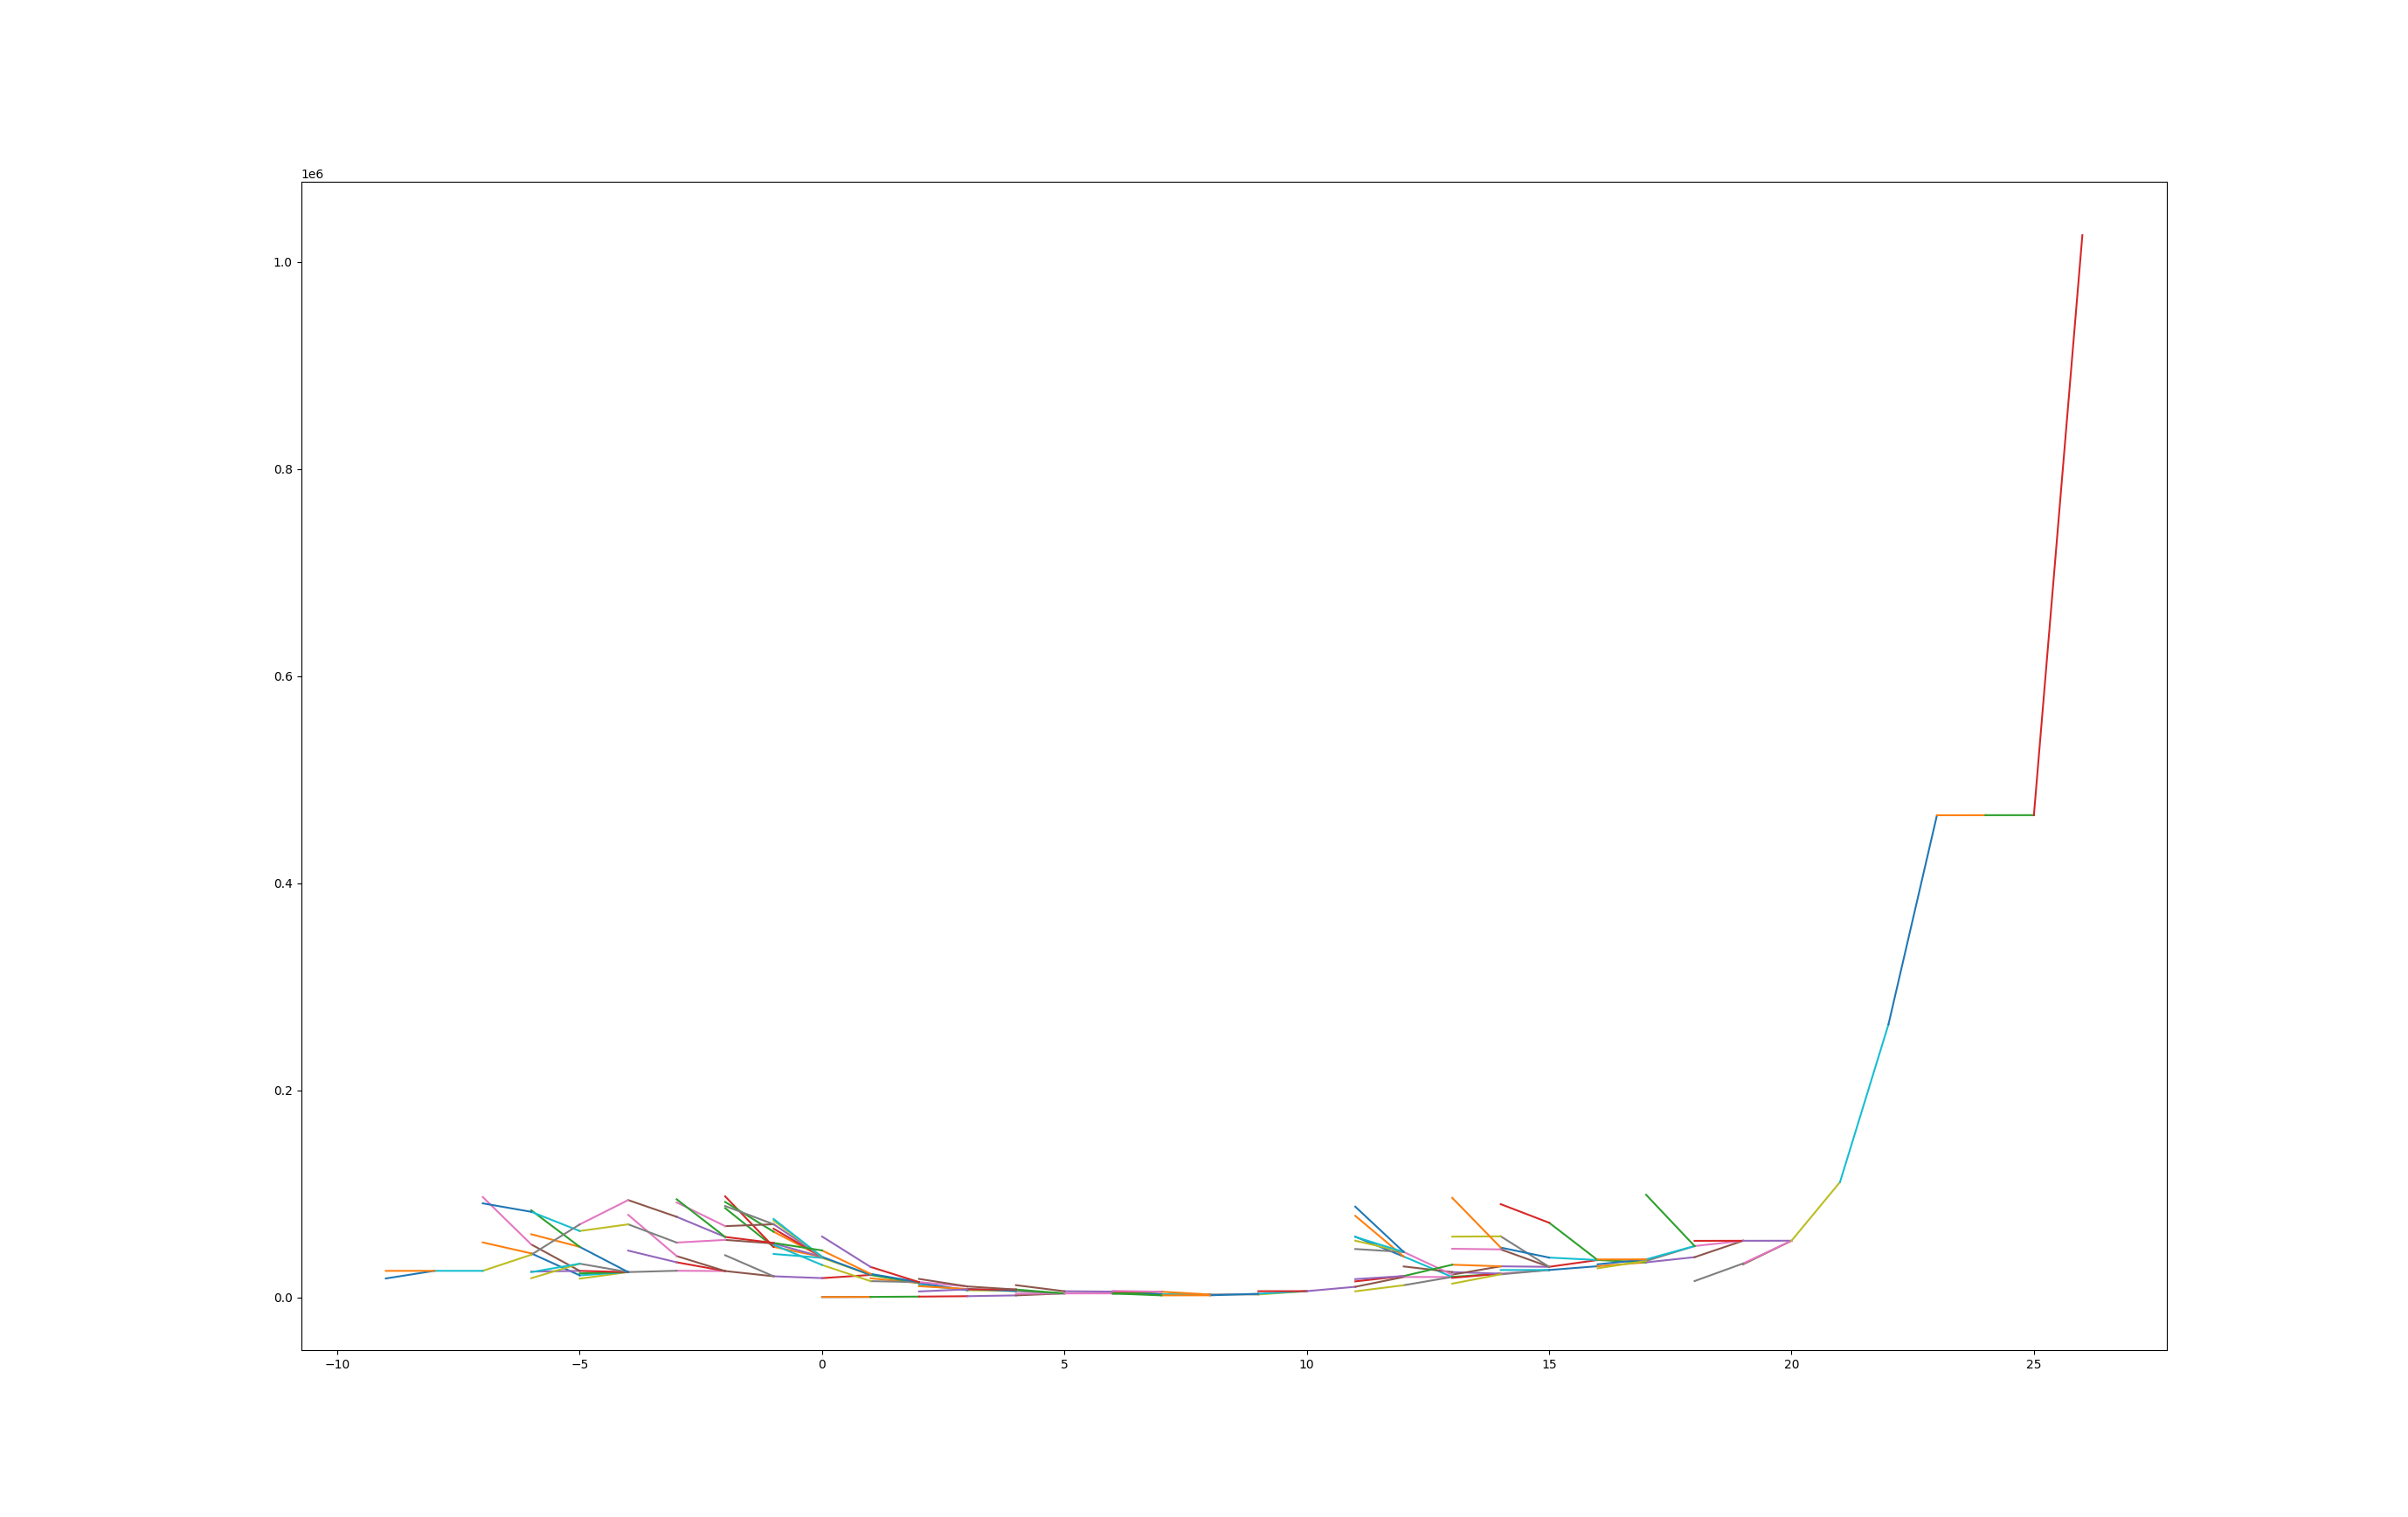
\includegraphics[width=1\textwidth]{aliq_276_max_1000000.png}
% \centering
% \end{figure}

\begin{figure}
  \makebox[\textwidth][c]{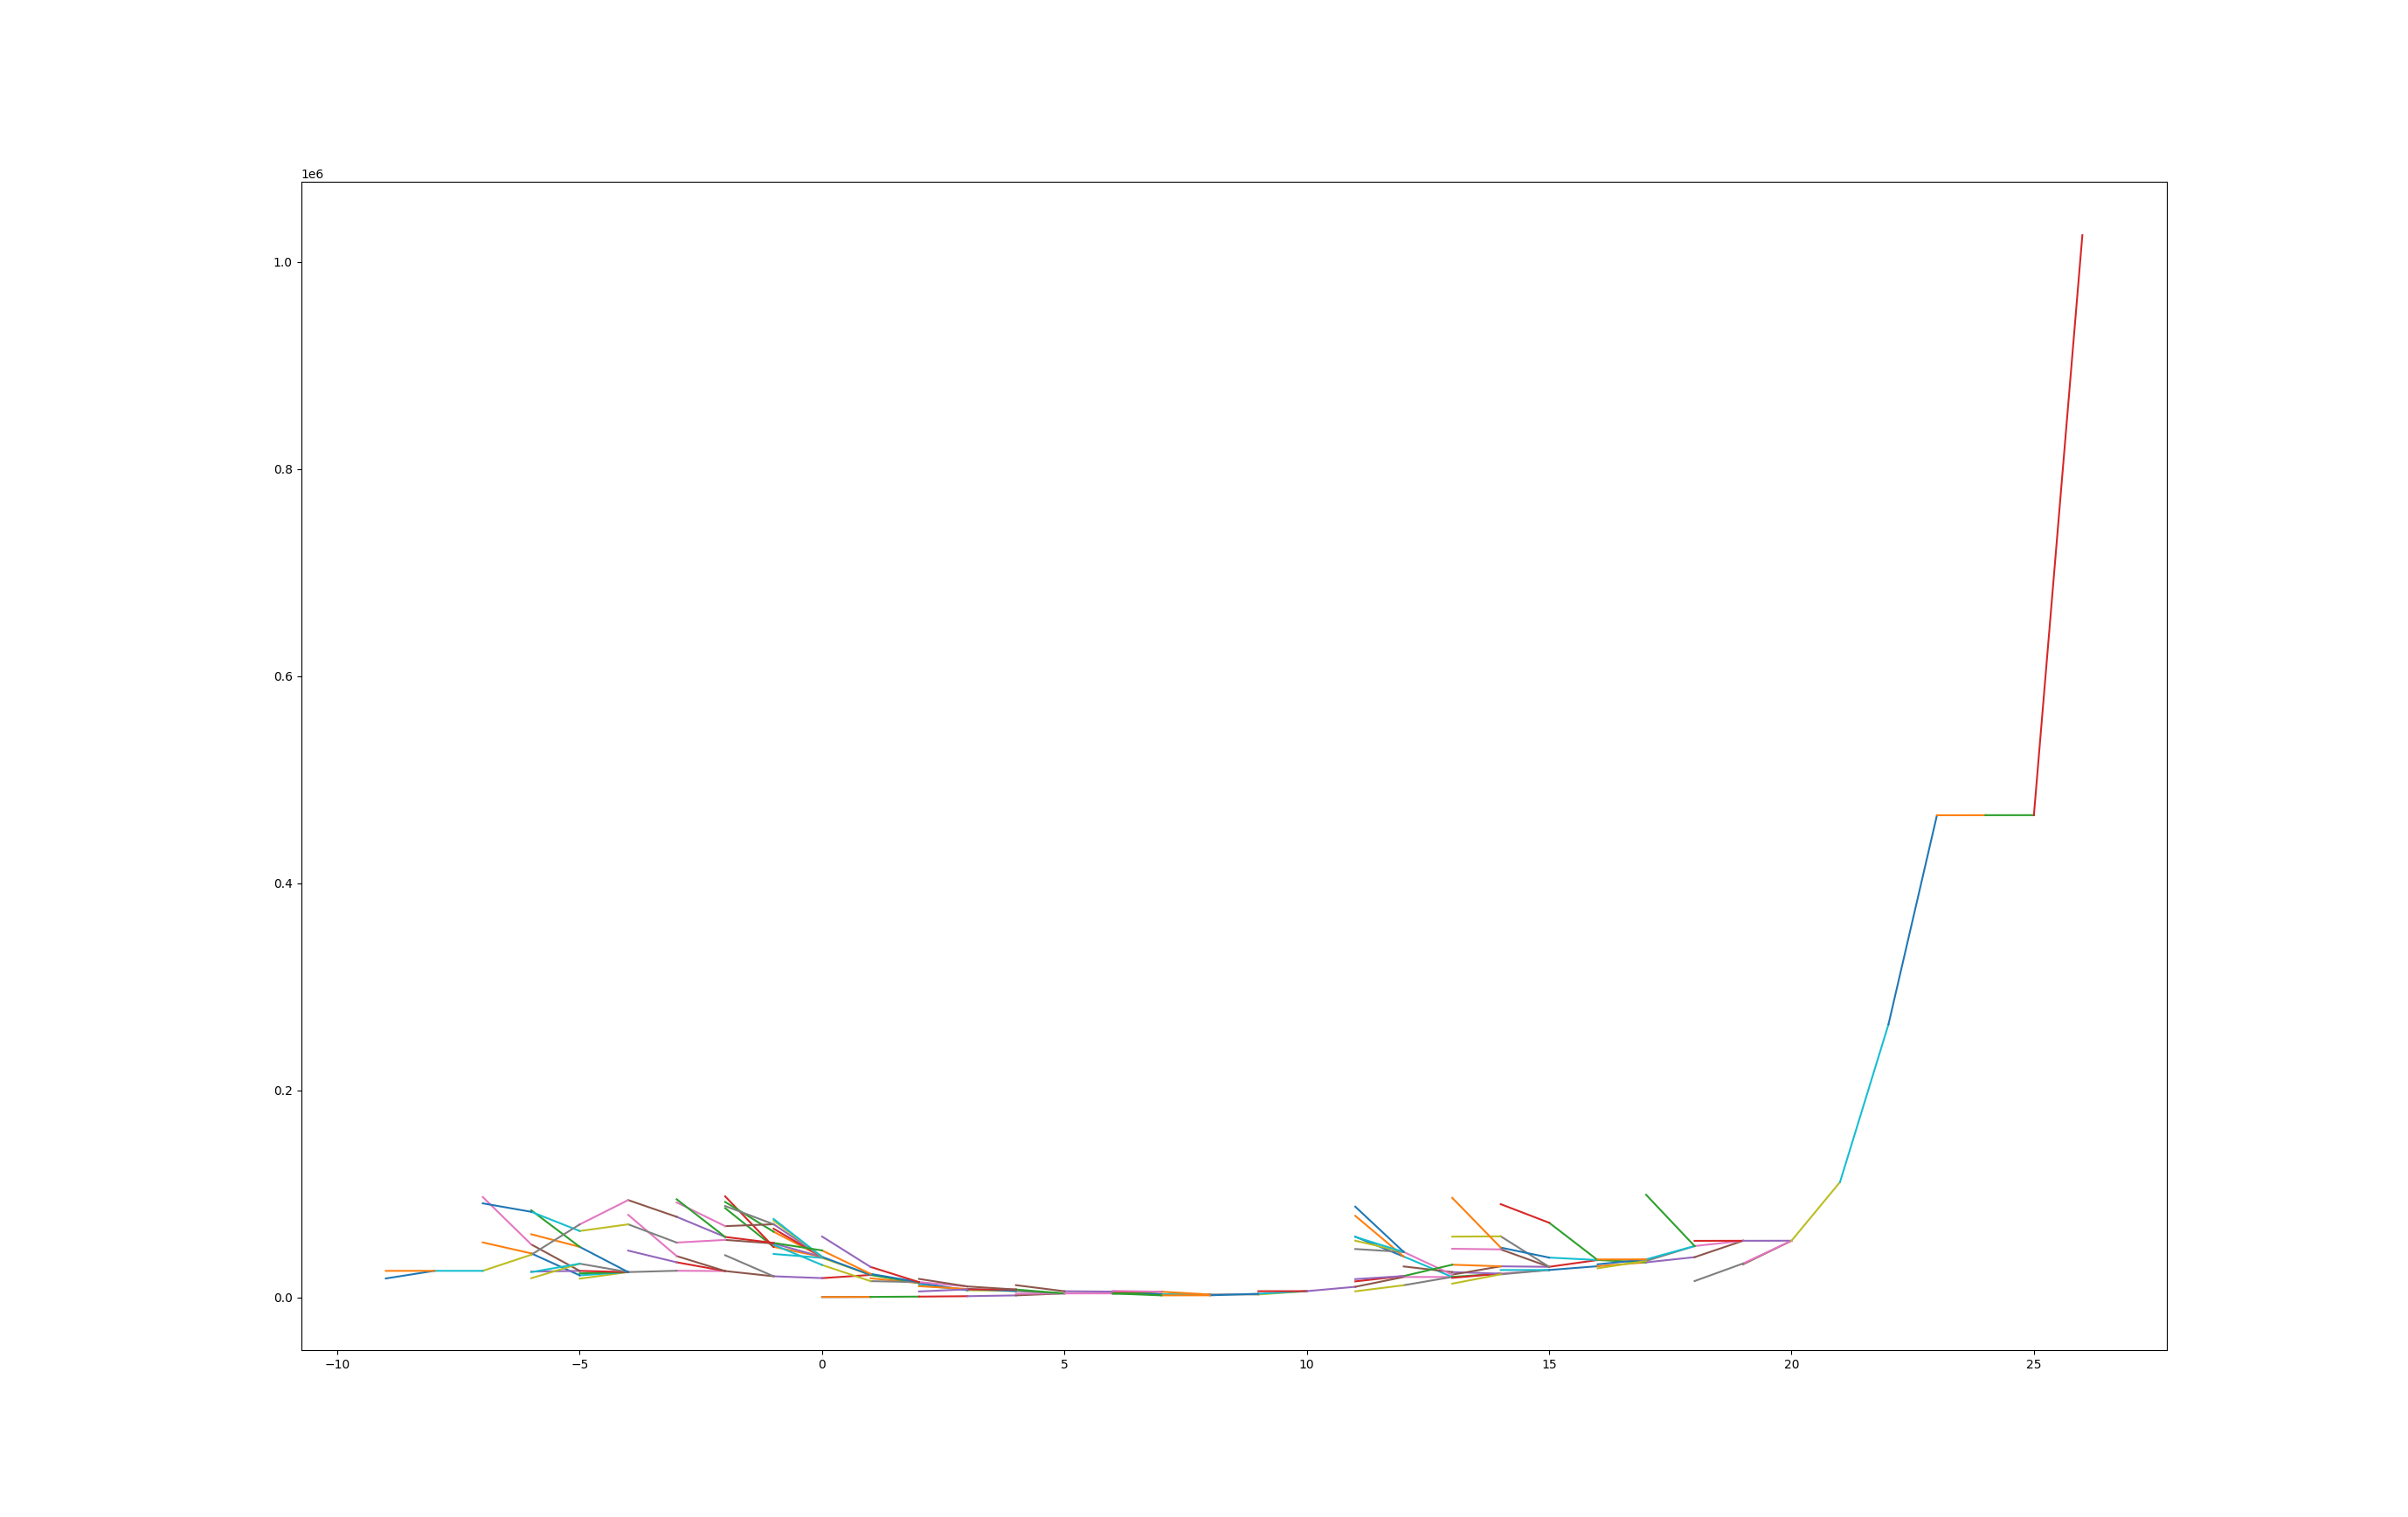
\includegraphics[width=2\textwidth]{aliq_276_max_1000000}}%
  \caption{Recursive plot of the 276 sequence's aliquot genealogy, the $x$ axis is the number of iterations before or after 276, the $y$ axis is the value of the aliquot number.}
  \label{fig:geno}
\end{figure}

%%%%%%%%%%%%%%%%%%%%%%%%%%%%%%%%%%%%%%%%
\bibliographystyle{apalike}
\bibliography{aliquot_proposal} 
\end{document}